\section{Finite Difference Method for Elliptic PDEs}

In case of a one-dimensional domain:
\begin{enumerate}
	\item Given the differential equation $Lu(x) = f(x)$
	\item{
		Discretise domain.
		E.g. we have $x_k^{(n)}=k\cdot\Delta x$ with $\Delta x = 1 / n$.
	}
	\item Discretise equation using discrete operators
	\item{
		Replace functions $u(x)$ and $f(x)$ by vectors of nodal values:
		$u_k^{(n)}=u\left(x_k^{(n)}\right)$ and $f_k^{(n)} = f\left(x_k^{(n)}\right)$
	}
	\item Solve for $A^{(n)}\cdot \tilde{u}^{(n)} = f^{(n)}$ for inner knots while considering boundary conditions.
\end{enumerate}

\subsection{One-Dimensional Example}

The boundary value problem $u''(x) = 4\cdot(u(x) - x)=4u(x)-4x,\quad x\in ]0,1[$ with $u(0) = 0$ and $u(1) = 2$
should be approximated by function $\tilde{u}(x)$ using FDM with $\Delta x = 1/4$.

The discretised equation therefore is:
\begin{align*}
	\frac{u_{k+1} - 2u_k + u_{k-1}}{\Delta x^2} = 4u_k - 4x_k\quad(k=1,\ldots,n-1)
\end{align*}

\makebox[\columnwidth]{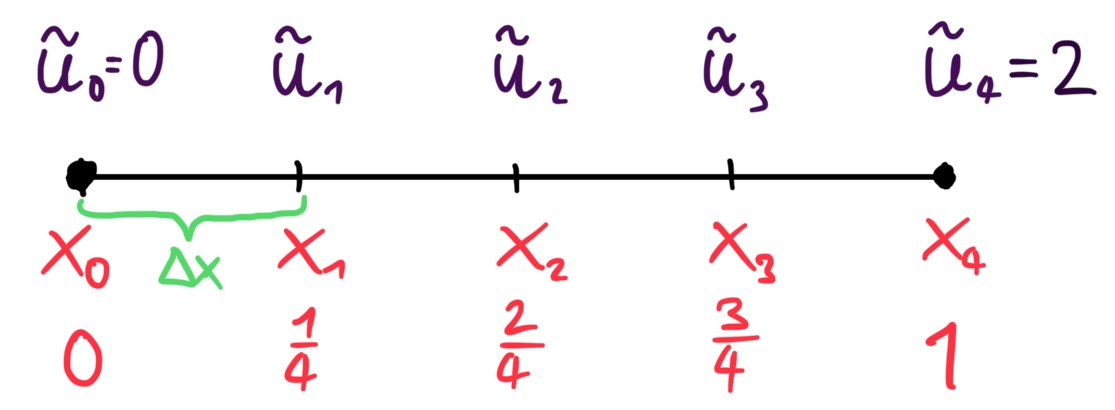
\includegraphics[width=0.6\columnwidth]{images/FDM_Elliptic}}

giving us the linear system
\begingroup
\renewcommand*{\arraystretch}{3}
  \begin{align*}
    \left|
    \begin{matrix}
      \frac{\tilde{u}_2 - 2\tilde{u}_1 + \cancelto{=0}{\tilde{u}_0}}{\cancelto{= 1/16}{\Delta x^2}} & = 4\tilde{u}_1 - 4\cancelto{1/4}{x_1} \\
      \frac{\tilde{u}_3 - 2\tilde{u}_2 + \tilde{u}_1}{\cancelto{= 1/16}{\Delta x^2}} & = 4\tilde{u}_2 - 4\cancelto{2/4}{x_2} \\
      \frac{\cancelto{= 2}{\tilde{u}_4} - 2\tilde{u}_3 + \tilde{u}_2}{\cancelto{= 1/16}{\Delta x^2}} & = 4\tilde{u}_3 - 4\cancelto{3/4}{x_3} \\
    \end{matrix}
    \right|
  \end{align*}
\endgroup

resulting in
\begin{align*}
	-32\utild_1 + 16\utild_2 & = 4\utild_1 - 1\quad\rightarrow -36\utild_1 + 16\utild_2 = -1 \\
	16\utild_1 - 32\utild_2 + 16\utild_3 & = 4\utild_2 - 2\quad\rightarrow 16\utild_1 - 36\utild_2 + 16\utild_3 = -2 \\
	16\utild_2 - 32\utild_3 + 16\cdot 2 & = 4\utild_3 - 3\quad\rightarrow 16\utild_2 - 36\utild_3 = -35
\end{align*}

ultimately giving the equation in matrix form (optional):
\begin{align*}
	\begin{bmatrix}
		-36 & 16 & 0 \\
		16 & -36 & 16 \\
		0 & 16 & -36
	\end{bmatrix}
	\cdot
	\begin{bmatrix}
		\utild_1 \\
		\utild_2 \\
		\utild_3 \\
	\end{bmatrix}
	=
	\begin{bmatrix}
		-1 \\
		-2 \\
		-35
	\end{bmatrix}
\end{align*}

giving the approximation vector $\utild \approx (0.4, 0.83, 1.34)$.

\subsection{Two-Dimensions Example}

We have Poisson's differential equation $-\Delta u(x,y)=f(x,y)$ with
$f(x,y) = \left( (3x+x^2)\cdot y(1-y) + (3y+y^2)\cdot x(1-x) \right)\cdot e^{x+y}$ on
$\Omega = [0,1]\times [0,1]$ with homogeneous boundary conditions.
Setting $h=\Delta x = \Delta y = \frac{1}{3}$, we can use the discrete Laplace operator.
Discretisation of the geometry yields
\makebox[\columnwidth]{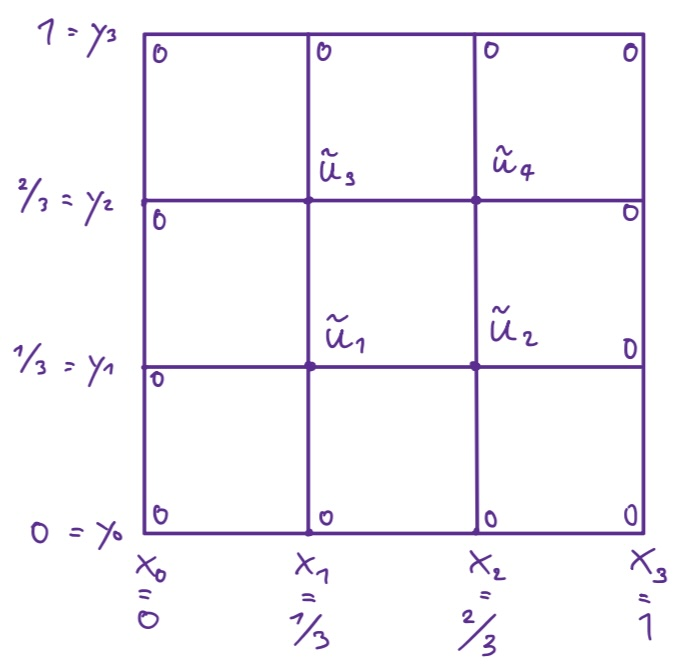
\includegraphics[width=0.5\columnwidth]{images/fdm_elliptic_2d}}

and we can define for each inner node an equation:
\begin{align*}
	u_1 & : -\frac{\utild_2 + \utild_3 + \cancelto{0}{y_1} + \cancelto{0}{x_1} - 4\utild_1}{\cancelto{(1/3)^2}{1/h^2}} = f(1/3, 1/3) = f_1 \\
	u_2 & : -\frac{0 + \utild_4 + \utild_1 + 0 - 4\utild_2}{(1/3)^2} = f(2/3, 1/3) = f_2 \\
	u_3 & : -\frac{\utild_4 + 0 + 0 + \utild_1 - 4\utild_3}{(1/3)^2} = f(1/3, 2/3) = f_3 \\
	u_4 & : -\frac{0 + 0 + \utild_3 + \utild_2 - 4\utild_4}{(1/3)^2} = f(2/3, 2/3) = f_4 \\
\end{align*}

giving the linear system:
\begin{align*}
	-9\cdot\begin{bmatrix}
		{\color{blue}-4} & {\color{blue}1} & {\color{purple}1} & {\color{purple}0} \\
		{\color{blue}1} & {\color{blue}-4} & {\color{purple}0} & {\color{purple}1} \\
		{\color{purple}1} & {\color{purple}0} & {\color{blue}-4} & {\color{blue}1} \\
		{\color{purple}0} & {\color{purple}1} & {\color{blue}1} & {\color{blue}-4}
	\end{bmatrix}
	\begin{bmatrix}
		\utild_1 \\
		\utild_2 \\
		\utild_3 \\
		\utild_4
	\end{bmatrix}
	=
	\begin{bmatrix}
		f_1 \\
		f_2 \\
		f_3 \\
		f_4
	\end{bmatrix}
\end{align*}
